\documentclass[12pt,a4paper]{article}

% ─── PACKAGES ───────────────────────────────────────────────────────────────
\usepackage[utf8]{inputenc}
\usepackage[T1]{fontenc}
\usepackage[english]{babel}
\usepackage{geometry}
\usepackage{graphicx}
\usepackage{booktabs}
\usepackage{array}
\usepackage{multirow}
\usepackage{amsmath}
\usepackage{hyperref}
\usepackage{xcolor}
\usepackage{listings}
\usepackage{caption}
\usepackage{subcaption}
\usepackage{float}
\usepackage{fancyhdr}
\usepackage{titlesec}
\usepackage{parskip}
\usepackage{microtype}
\usepackage{enumitem}
\usepackage{cite}

% ─── PAGE GEOMETRY ──────────────────────────────────────────────────────────
\geometry{a4paper, top=2.5cm, bottom=2.5cm, left=2.5cm, right=2.5cm}

% ─── COLORS ─────────────────────────────────────────────────────────────────
\definecolor{codeblue}{RGB}{0, 102, 204}
\definecolor{codegray}{RGB}{128, 128, 128}
\definecolor{codegreen}{RGB}{0, 153, 0}
\definecolor{backgray}{RGB}{245, 245, 245}
\definecolor{headerblue}{RGB}{0, 70, 127}

% ─── CODE LISTING STYLE ─────────────────────────────────────────────────────
\lstset{
    backgroundcolor=\color{backgray},
    basicstyle=\ttfamily\small,
    keywordstyle=\color{codeblue}\bfseries,
    commentstyle=\color{codegreen}\itshape,
    stringstyle=\color{codegray},
    breaklines=true,
    frame=single,
    numbers=left,
    numberstyle=\tiny\color{codegray},
    numbersep=5pt,
    showspaces=false,
    showstringspaces=false,
    tabsize=4,
    captionpos=b
}

% ─── HEADER / FOOTER ────────────────────────────────────────────────────────
\pagestyle{fancy}
\fancyhf{}
\fancyhead[L]{\small\textcolor{headerblue}{CENG 467 – NLU\&G Take-Home Midterm}}
\fancyhead[R]{\small\textcolor{headerblue}{Student ID: \studentid}}
\fancyfoot[C]{\thepage}
\renewcommand{\headrulewidth}{0.4pt}

% ─── SECTION FORMATTING ─────────────────────────────────────────────────────
\titleformat{\section}
    {\large\bfseries\color{headerblue}}
    {Question \thesection.}{0.5em}{}[\titlerule]
\titleformat{\subsection}{\normalsize\bfseries}{\thesubsection}{0.5em}{}

% ─── CUSTOM COMMANDS ────────────────────────────────────────────────────────
\newcommand{\studentid}{310201089}
\newcommand{\studentname}{Zehra Eda Cesur}
\newcolumntype{C}[1]{>{\centering\arraybackslash}p{#1}}

% ─── HYPERREF SETUP ─────────────────────────────────────────────────────────
\hypersetup{colorlinks=true, linkcolor=headerblue,
            urlcolor=codeblue, citecolor=codegreen}

% ════════════════════════════════════════════════════════════════════════════
\begin{document}
% ════════════════════════════════════════════════════════════════════════════

% ─── TITLE PAGE ─────────────────────────────────────────────────────────────
% ─── TITLE PAGE ─────────────────────────────────────────────────────────────
\begin{titlepage}
    \begin{center}
    \vspace*{1cm}
    
    {\Large\bfseries Izmir Institute of Technology\\[0.3em]
    Department of Computer Engineering}
    
    \vspace{1.5cm}
    
    \noindent\rule{\linewidth}{1pt}\\[0.4cm]
    
    {\LARGE\bfseries\color{headerblue}
        CENG 467 – Natural Language\\[0.3em]
        Understanding and Generation\\[0.4cm]
        Take-Home Midterm Examination}\\[0.4cm]
        
    \noindent\rule{\linewidth}{1pt}
    
    \vspace{1.5cm}
    
    \begin{tabular}{rl}
        \textbf{Student Name:} & \studentname \\[0.4em]
        \textbf{Student ID:}   & \studentid   \\[0.4em]
        \textbf{Instructor:}   & Prof.\ Dr.\ Aytu\u{g} Onan \\[0.4em]
        \textbf{Deadline:}     & 30 Nisan 2026, 23:59 \\
    \end{tabular}
    
    \vspace{1.5cm}

    \textbf{GitHub Repository:}\\[0.3em]
    \url{https://github.com/zedaeda/CENG467-takeHomeMidterm}

    \vfill
    {\small Spring 2026}
    \end{center}
\end{titlepage}

% ════════════════════════════════════════════════════════════════════════════
\section{Representation Learning in Text Classification}
% ════════════════════════════════════════════════════════════════════════════

\subsection{Dataset Description}

For this question, the IMDb Large Movie Review Dataset \cite{maas2011imdb} was
chosen for binary sentiment classification. The dataset contains movie reviews
from the IMDb platform, each labeled as \textit{positive} or \textit{negative}
based on the user's star rating.

Since the experiments were run on Google Colab's free tier with limited GPU
resources, a subset of the full dataset was used: 5{,}000 samples for training,
1{,}000 for validation, and 2{,}000 for testing. As shown in
Table~\ref{tab:q1_dataset}, the class distribution is nearly balanced across
all splits, which means the results are not affected by class imbalance.

\begin{table}[H]
    \centering
    \caption{IMDb Dataset Statistics (Subset Used in Experiments)}
    \begin{tabular}{lccc}
        \toprule
        \textbf{Split} & \textbf{Samples} & \textbf{Positive} & \textbf{Negative} \\
        \midrule
        Train      & 5{,}000 & 2{,}506 & 2{,}494 \\
        Validation & 1{,}000 &    488  &    512  \\
        Test       & 2{,}000 & 1{,}001 &    999  \\
        \bottomrule
    \end{tabular}
    \label{tab:q1_dataset}
\end{table}

\subsection{Preprocessing Pipeline and Tokenization}

A common preprocessing pipeline was applied to all models where possible.
Raw texts were lowercased and non-alphabetic characters were removed using
regular expressions. Sequences longer than 256 tokens were truncated.

Two different tokenization strategies were compared:

\textbf{Strategy A — Word-level tokenization (TF-IDF and BiLSTM):}
A simple whitespace and punctuation-based tokenizer was used, keeping only
tokens with at least two characters. This approach is fast and easy to
understand, but it cannot handle rare or unseen words well.

\textbf{Strategy B — WordPiece tokenization (DistilBERT):}
The pre-trained \\ \texttt{distilbert-base-uncased} tokenizer splits unknown words
into smaller known subword units (e.g., \textit{``playing''} $\rightarrow$
\textit{``play''} + \textit{``\#\#ing''}). This eliminates out-of-vocabulary
problems and preserves more morphological information. Sequences were padded or
truncated to 128 tokens.

The main difference between these two strategies is that WordPiece gives richer
representations for rare words, while word-level tokenization is much faster
and simpler.

\subsection{Model Implementations}

\subsubsection{TF-IDF + Logistic Regression (Sparse Baseline)}

Two TF-IDF configurations were tested: unigram only $(1,1)$ with 20{,}000
features, and unigram+bigram $(1,2)$ with 30{,}000 features, both using
sublinear TF scaling. A Logistic Regression classifier with $C{=}1.0$ was
trained on these sparse vectors. The bigram configuration performed better on 
validation (Accuracy: 0.860 vs.\ 0.847) and was selected for \footnote{Code and report writing assistance was provided by
Claude \cite{claude2026} and Gemini \cite{gemini2026}.} the  final evaluation.


\subsubsection{BiLSTM (Dense Neural Baseline)}

A two-layer Bidirectional LSTM was implemented from scratch in PyTorch.
Word embeddings of dimension 128 were randomly initialized and trained together
with the model. The LSTM had a hidden size of 256 per direction, with 0.3
dropout. Training ran for 5 epochs using Adam (lr = $10^{-3}$), gradient
clipping at 1.0, and a batch size of 64.

\subsubsection{DistilBERT (Contextual Transformer)}

The \texttt{distilbert-base-uncased} checkpoint \cite{devlin2019bert} was
fine-tuned for sentiment classification by adding a classification head on top
of the pre-trained encoder. Fine-tuning ran for 3 epochs with AdamW
(lr = $2 \times 10^{-5}$, weight decay = 0.01), a linear warmup over 10\% of
steps, and a batch size of 32.

\subsection{Results}

The test set results are shown in Table~\ref{tab:q1_results}, and a visual
comparison is given in Figure~\ref{fig:q1_comparison}.

\begin{table}[H]
    \centering
    \caption{Text Classification Results (Test Set)}
    \begin{tabular}{lC{2.5cm}C{2.5cm}C{2.5cm}}
        \toprule
        \textbf{Model} & \textbf{Accuracy (\%)} & \textbf{Macro-F1 (\%)} & \textbf{Training Time} \\
        \midrule
        TF-IDF + LR  & 87.25 & 87.25 & $\sim$2 min  \\
        BiLSTM        & 68.95 & 68.94 & $\sim$10 min \\
        DistilBERT    & 86.60 & 86.60 & $\sim$25 min \\
        \bottomrule
    \end{tabular}
    \label{tab:q1_results}
\end{table}

\begin{figure}[H]
    \centering
    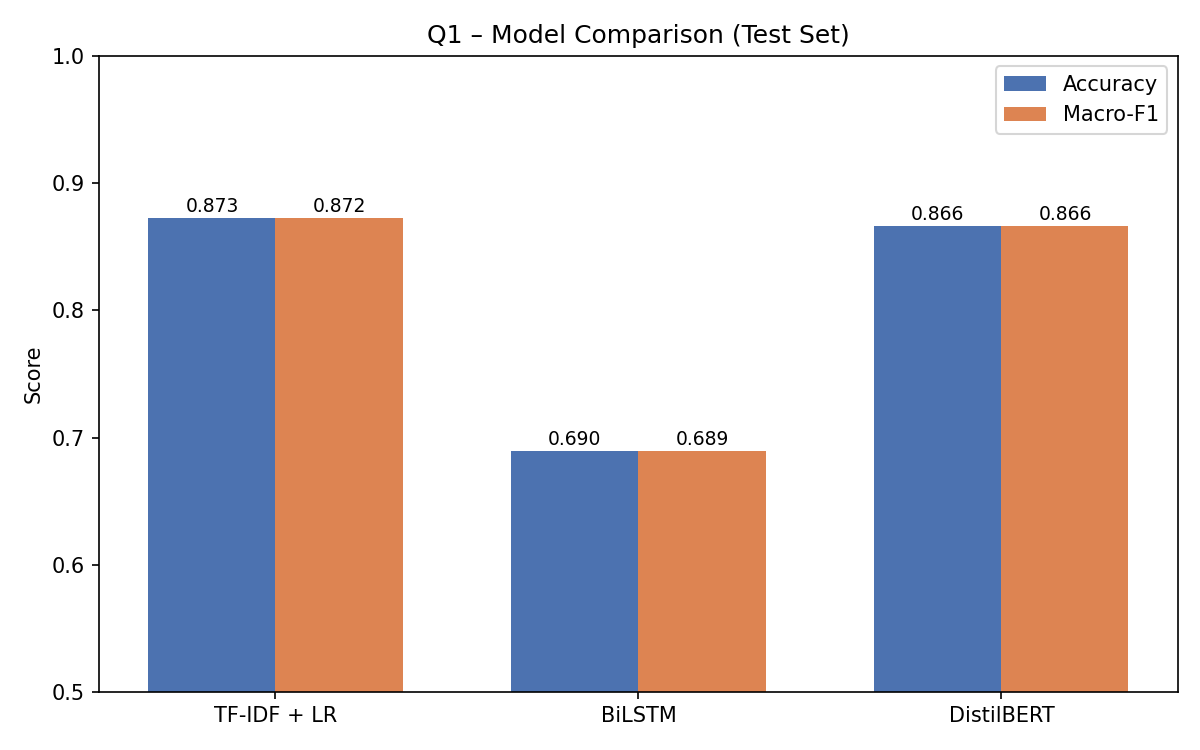
\includegraphics[width=0.75\linewidth]{figures/q1_comparison.png}
    \caption{Accuracy and Macro-F1 comparison across the three models on the test set.}
    \label{fig:q1_comparison}
\end{figure}

\begin{figure}[H]
    \centering
    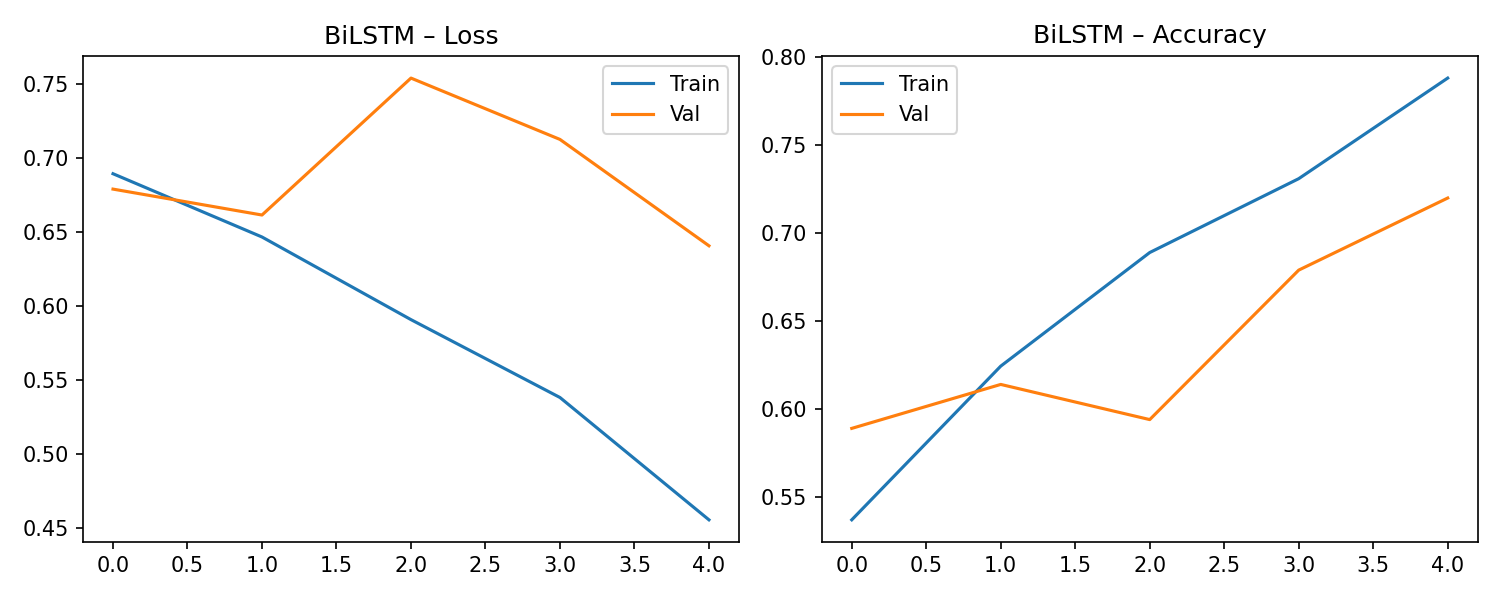
\includegraphics[width=0.95\linewidth]{figures/q1_bilstm_training.png}
    \caption{BiLSTM training and validation loss/accuracy over 5 epochs.
             The gap between train and validation loss after epoch 2 is a
             sign of overfitting.}
    \label{fig:q1_bilstm_train}
\end{figure}

\subsection{Error Analysis}

Table~\ref{tab:q1_errors} shows five misclassified examples, and
Figure~\ref{fig:q1_cms} shows the confusion matrices for all three models.

\begin{table}[H]
    \centering
    \caption{Representative Misclassified Examples}
    \begin{tabular}{p{6.5cm}ccp{3cm}}
        \toprule
        \textbf{Text (truncated)} & \textbf{True} & \textbf{Pred.} & \textbf{Error Type} \\
        \midrule
        ``Unfortunately, my old Blockbuster thought it was a good idea to have the sequel...'' &
        Pos & Neg & Context loss \\[4pt]
        ``I must assume the role of the turd in the punchbowl...encomia of praise...'' &
        Neg & Pos & Irony / sarcasm \\[4pt]
        ``real evidence of what a misguided and unchecked government can do...'' &
        Pos & Neg & Domain shift \\[4pt]
        ``Lucille Ball was a mighty power in television...but she still made an occasional film...'' &
        Neg & Pos & Misleading opening \\[4pt]
        ``I was Stan in the movie. Stan was the friend that...got his arm smashed...'' &
        Neg & Pos & Ambiguous narrative \\
        \bottomrule
    \end{tabular}
    \label{tab:q1_errors}
\end{table}

\begin{figure}[H]
    \centering
    \begin{subfigure}[b]{0.32\textwidth}
        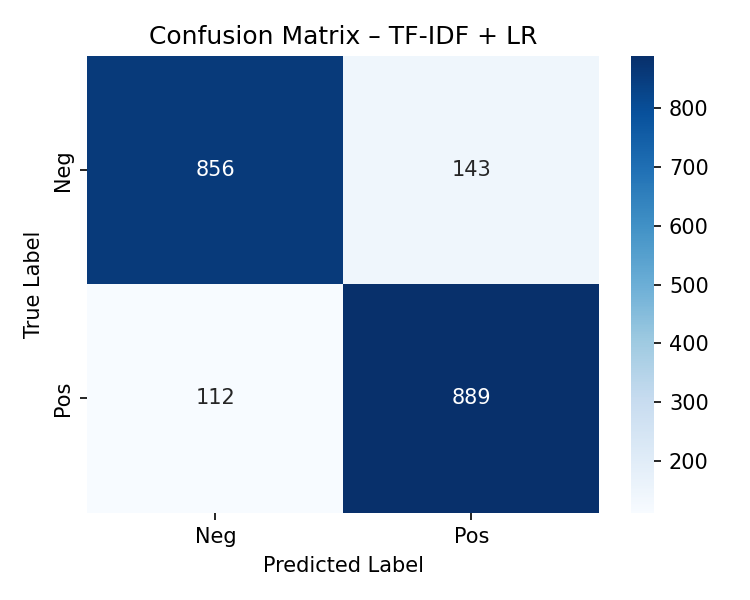
\includegraphics[width=\linewidth]{figures/q1_cm_tfidf.png}
        \caption{TF-IDF + LR}
    \end{subfigure}
    \begin{subfigure}[b]{0.32\textwidth}
        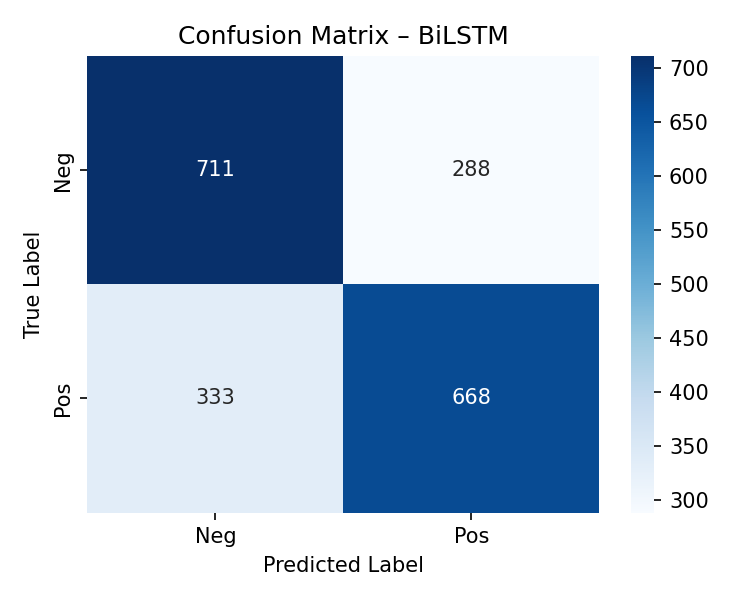
\includegraphics[width=\linewidth]{figures/q1_cm_bilstm.png}
        \caption{BiLSTM}
    \end{subfigure}
    \begin{subfigure}[b]{0.32\textwidth}
        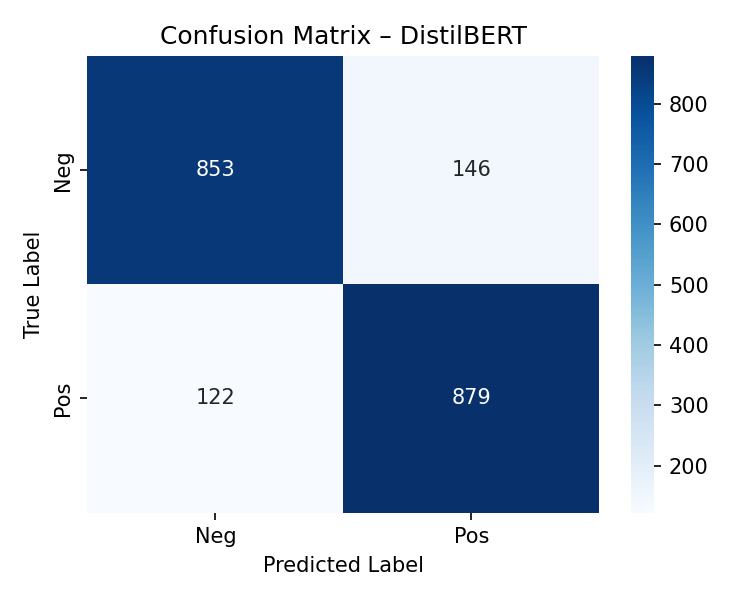
\includegraphics[width=\linewidth]{figures/q1_cm_bert.png}
        \caption{DistilBERT}
    \end{subfigure}
    \caption{Confusion matrices for all three models on the test set.}
    \label{fig:q1_cms}
\end{figure}

Looking at the errors, five common patterns stood out:

\textbf{(1) Context loss:} TF-IDF and BiLSTM struggled with reviews where the
overall sentiment depends on the full narrative rather than individual words.
A review starting with ``unfortunately'' about a missing film was labeled
negative, even though the reviewer actually praised both films.

\textbf{(2) Irony and sarcasm:} Phrases like ``encomia of praise'' were used
ironically, but all models treated them as positive signals. This kind of
pragmatic reasoning is very hard for current models.

\textbf{(3) Domain shift:} Reviews about politically-charged topics used
negative-sounding words like ``misguided government'' to describe film content,
not the film quality itself. All three models were confused by this.

\textbf{(4) Misleading opening sentences:} Some negative reviews began with
long positive descriptions of an actor or director, and only turned critical
later. Models that focus heavily on early tokens were tricked by this pattern.

\textbf{(5) Ambiguous narratives:} Reviews written from a personal perspective
(e.g., someone who acted in the film) did not have clear positive or negative
signals, making correct classification difficult even for humans.

\subsection{Discussion}

The results were quite interesting and somewhat unexpected. The simplest model,
TF-IDF + LR, actually performed the best (87.25\%), while the more complex
BiLSTM came in last (68.95\%). 

\textbf{Why did TF-IDF win?} With only 5{,}000 training examples, TF-IDF has
a natural advantage: it does not need to learn anything from scratch. It simply
counts word frequencies, which works surprisingly well for sentiment analysis
where words like ``terrible'' or ``amazing'' are strong indicators. The BiLSTM,
on the other hand, had to learn word meanings from scratch with very limited
data, which led to clear overfitting.

\textbf{Why did BiLSTM underperform?} The training loss kept going down while
the validation loss went up after epoch 2. This is a textbook case of
overfitting. With the full 25{,}000-sample dataset, BiLSTM would likely
perform much better.

\textbf{What about DistilBERT?} DistilBERT came very close to TF-IDF (86.60\%)
despite being fine-tuned on the same small subset. This shows the power of
transfer learning — the model already knows a lot about language from its
pre-training, so it needs less task-specific data. Its confusion matrix also
shows the fewest total errors (268 vs.\ 621 for BiLSTM), meaning its mistakes
are fewer even if its accuracy is similar to TF-IDF.

Regarding the effect of preprocessing decisions, stopword removal
was applied during TF-IDF vectorization but not for BiLSTM or BERT,
as neural models can learn to ignore uninformative tokens. Truncation
at 256 tokens for BiLSTM and 128 for DistilBERT had minimal impact
given that average review length was well within these limits.

In summary, for small datasets, simple methods can be surprisingly effective.
But as data grows, contextual models like BERT are expected to pull ahead
significantly \cite{devlin2019bert}.

% ════════════════════════════════════════════════════════════════════════════
\section{Named Entity Recognition}
% ════════════════════════════════════════════════════════════════════════════

\subsection{Dataset Description and BIO Tagging}

The CoNLL-2003 dataset \cite{tjong2003conll} was used for this task. It is one
of the most widely-used benchmarks for Named Entity Recognition (NER). The
dataset labels each token with one of four entity types: Person (\textbf{PER}),
Organization (\textbf{ORG}), Location (\textbf{LOC}), and Miscellaneous
(\textbf{MISC}).

The annotations follow the BIO tagging scheme (Begin, Inside, Outside),
which in theory gives 9 unique tags: \texttt{O}, \texttt{B-PER},
\texttt{I-PER}, \texttt{B-ORG}, \texttt{I-ORG}, \texttt{B-LOC},
\texttt{I-LOC}, \texttt{B-MISC}, and \texttt{I-MISC}. In our downloaded
version of the dataset, only \texttt{I-} prefixes were present (no \texttt{B-}
prefixes), so 8 unique tags were used in practice.

For the BERT model, subword tokenization creates an alignment problem: a single
word like ``Washington'' might be split into multiple tokens. To handle this,
only the first subtoken of each word was assigned the original NER label. The
remaining subtokens were assigned a dummy label (\texttt{-100}) that is ignored
during loss computation.

\begin{table}[H]
    \centering
    \caption{CoNLL-2003 Dataset Statistics}
    \begin{tabular}{lccc}
        \toprule
        \textbf{Split} & \textbf{Sentences} & \textbf{Tokens} & \textbf{Entities} \\
        \midrule
        Train      & 14{,}041 & 203{,}621 & 23{,}499 \\
        Validation &  3{,}250 &  51{,}362 &  5{,}942 \\
        Test       &  3{,}453 &  46{,}435 &  5{,}648 \\
        \bottomrule
    \end{tabular}
    \label{tab:q2_dataset}
\end{table}

\subsection{Model Implementations}

\subsubsection{BiLSTM-CRF (Hybrid Architecture)}

The first model combines a Bidirectional LSTM with a Conditional Random Field
(CRF) layer \cite{lafferty2001crf,lample2016bilstmcrf}. The BiLSTM reads each
token in both directions and produces context-aware representations, while the
CRF layer uses transition probabilities between tags to prevent invalid label
sequences (e.g., going directly from \texttt{O} to \texttt{I-PER} is penalized).

Word embeddings of dimension 100 were randomly initialized and trained from
scratch. The BiLSTM had a hidden dimension of 128. The model has approximately
2M parameters and was trained for 10 epochs with Adam (lr = $10^{-3}$).

\subsubsection{BERT for Token Classification}

The second model uses \texttt{distilbert-base-uncased} \cite{devlin2019bert}
with a linear token classification head on top. It was fine-tuned for 3 epochs
with AdamW (lr = $5 \times 10^{-5}$) and a linear learning rate scheduler with
warmup. The model has approximately 66.3M parameters.

\subsection{Results}

\begin{table}[H]
    \centering
    \caption{NER Results per Entity Type (Test Set)}
    \begin{tabular}{lC{2cm}C{2cm}C{2cm}C{2cm}}
        \toprule
        \textbf{Model / Entity} & \textbf{Precision} & \textbf{Recall} & \textbf{F1} & \textbf{Support} \\
        \midrule
        \multicolumn{5}{l}{\textit{BiLSTM-CRF}} \\
        \quad PER  & 0.0212 & 0.0155 & 0.0179 & 1617 \\
        \quad ORG  & 0.1062 & 0.0566 & 0.0738 & 1661 \\
        \quad LOC  & 0.1248 & 0.1145 & 0.1194 & 1668 \\
        \quad MISC & 0.0773 & 0.0627 & 0.0692 &  702 \\
        \quad \textbf{Overall} & \textbf{0.0851} & \textbf{0.0627} & \textbf{0.0722} & \textbf{5648} \\
        \midrule
        \multicolumn{5}{l}{\textit{BERT-NER}} \\
        \quad PER  & 0.9647 & 0.9635 & 0.9641 & 1616 \\
        \quad ORG  & 0.8810 & 0.8736 & 0.8773 & 1661 \\
        \quad LOC  & 0.9047 & 0.9286 & 0.9165 & 1667 \\
        \quad MISC & 0.7590 & 0.8077 & 0.7826 &  702 \\
        \quad \textbf{Overall} & \textbf{0.8958} & \textbf{0.9074} & \textbf{0.9015} & \textbf{5646} \\
        \bottomrule
    \end{tabular}
    \label{tab:q2_results}
\end{table}

\begin{figure}[H]
    \centering
    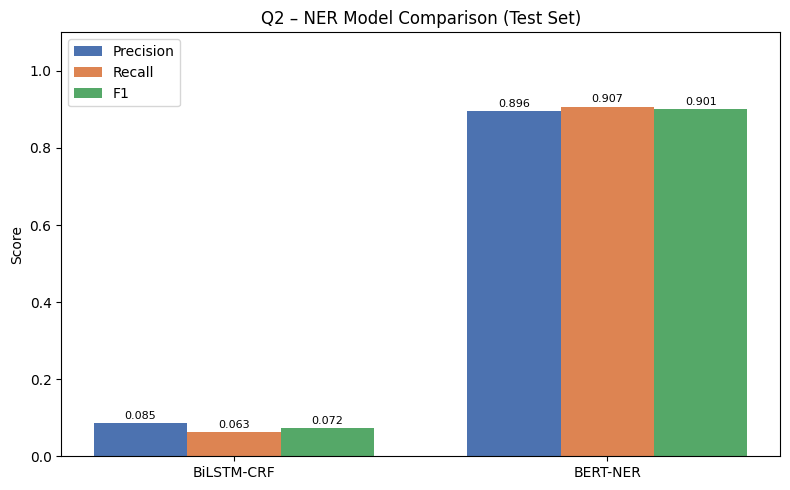
\includegraphics[width=0.75\linewidth]{figures/q2_comparison.png}
    \caption{Precision, Recall, and F1 comparison between BiLSTM-CRF and
             BERT-NER on the CoNLL-2003 test set.}
    \label{fig:q2_comparison}
\end{figure}

\begin{figure}[H]
    \centering
    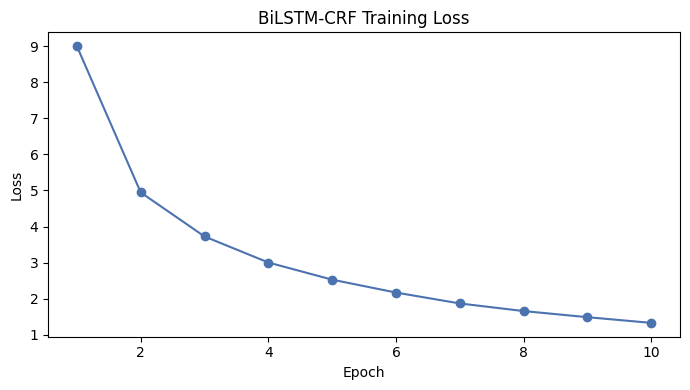
\includegraphics[width=0.65\linewidth]{figures/q2_crf_loss.png}
    \caption{BiLSTM-CRF training loss over 10 epochs.}
    \label{fig:q2_crf_loss}
\end{figure}

\subsection{Error Analysis and Discussion}

The gap between the two models was very large: BERT-NER reached an overall F1
of 0.90, while BiLSTM-CRF only reached 0.07. This was the most striking result
of the entire midterm for me, so I want to explain it carefully.

The BiLSTM-CRF's poor performance comes down to one main reason: its embeddings
were initialized randomly and trained from scratch on the CoNLL data alone. The
standard practice for BiLSTM-CRF is to initialize embeddings with pre-trained
GloVe vectors, which already encode word meanings \cite{lample2016bilstmcrf}.
Without this, the model had no prior knowledge of what words mean, so it mostly
predicted \texttt{O} for everything and occasionally guessed wrong entity types.
For example, it predicted commas as \texttt{I-LOC} and missed obvious entities
like ``JAPAN''.

BERT's errors were much more interesting. For instance, it labeled ``CHINA'' as
\texttt{I-LOC} in the sentence ``CHINA IN SURPRISE DEFEAT'', when the dataset
labeled it as \texttt{I-PER} (referring to a sports team). BERT was not wrong
in a linguistic sense — it simply applied its geographic prior instead of
understanding the sports context. It also occasionally missed \texttt{MISC}
entities like ``1995'' in ``1995 World Cup''.

These results confirm that pre-trained contextual embeddings are essential for
NER. The CRF layer helps enforce valid tag sequences, but it cannot make up for
the lack of good token representations.

% ════════════════════════════════════════════════════════════════════════════
\section{Text Summarization}
% ════════════════════════════════════════════════════════════════════════════

\subsection{Dataset Description}

The CNN/DailyMail dataset \cite{hermann2015cnndm} was used for this task.
It pairs news articles with human-written bullet-point summaries, making it a
standard benchmark for summarization. Due to computational constraints, only
500 randomly sampled articles from the test split were used for evaluation.

\begin{table}[H]
    \centering
    \caption{CNN/DailyMail Subset Statistics}
    \begin{tabular}{lc}
        \toprule
        \textbf{Property} & \textbf{Value} \\
        \midrule
        Subset size (test)            & 500 articles \\
        Avg.\ article length          & 687 words \\
        Avg.\ reference summary length & 56 words \\
        \bottomrule
    \end{tabular}
    \label{tab:q3_dataset}
\end{table}

\subsection{Model Implementations}

\subsubsection{TextRank (Extractive)}

TextRank \cite{mihalcea2004textrank} is a graph-based algorithm adapted from
PageRank. Each sentence is a node, and edges are weighted by the overlap between
sentences (shared non-stopword tokens, normalized by sentence length). A damping
factor of 0.85 was used, with convergence tolerance $10^{-6}$ and a maximum of
100 iterations. The top-3 ranked sentences, in their original order, form the
summary. TextRank runs entirely on CPU and needs no training data.

\subsubsection{BART (Abstractive)}

BART \cite{lewis2020bart} is a sequence-to-sequence transformer pre-trained
with a denoising objective. The \texttt{facebook/bart-large-cnn} checkpoint was
used directly without additional fine-tuning, since it was already fine-tuned
on CNN/DailyMail. Articles were truncated to 3{,}000 characters before being
fed to the model. Summaries were generated with greedy decoding, a maximum
length of 130 tokens, and a minimum of 30 tokens.

\subsection{Quantitative Results}

\begin{table}[H]
    \centering
    \caption{Summarization Evaluation Results (500-sample Test Subset)}
    \begin{tabular}{lC{2cm}C{2cm}}
        \toprule
        \textbf{Metric} & \textbf{TextRank} & \textbf{BART} \\
        \midrule
        ROUGE-1   & 0.3559 & \textbf{0.4380} \\
        ROUGE-2   & 0.1392 & \textbf{0.2121} \\
        ROUGE-L   & 0.2279 & \textbf{0.3082} \\
        BLEU      & 0.0923 & \textbf{0.1810} \\
        METEOR    & 0.3419 & \textbf{0.3817} \\
        BERTScore & 0.8653 & \textbf{0.8819} \\
        \bottomrule
    \end{tabular}
    \label{tab:q3_results}
\end{table}

\begin{figure}[H]
    \centering
    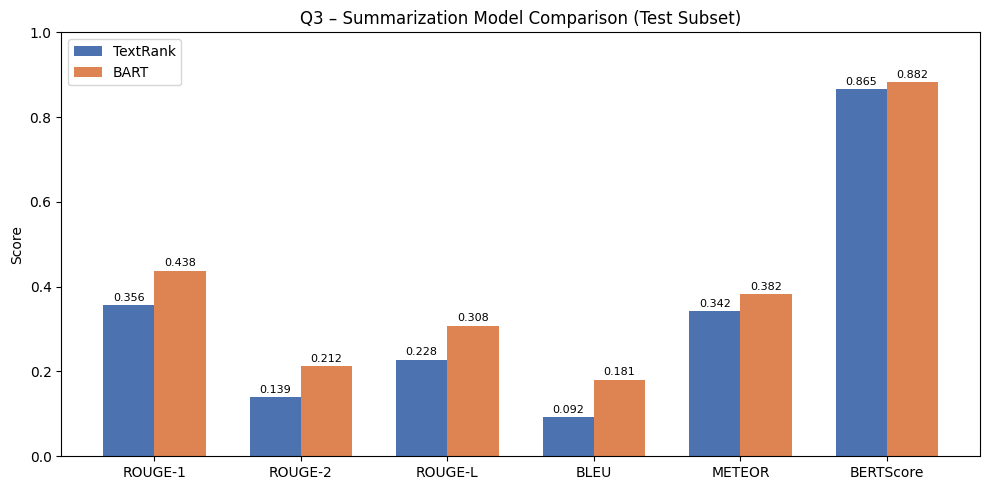
\includegraphics[width=0.85\linewidth]{figures/q3_comparison.png}
    \caption{Metric-by-metric comparison of TextRank and BART on the
             CNN/DailyMail test subset.}
    \label{fig:q3_comparison}
\end{figure}

\subsection{Qualitative Examples}

\textbf{Example 1 — Medical Marijuana Article}\\
\textit{Reference:} CNN's Dr.\ Sanjay Gupta argues for legalizing medical
marijuana, acknowledging his own inaction on the issue.\\
\textit{TextRank:} Picked three sentences from the article body, capturing the
political context but missing the author's personal stance and the key statistic
(53\% majority support).\\
\textit{BART:} Correctly named the author, included the 53\% figure, and
summarized the trend concisely.\\
\textit{Analysis:} BART was better at pulling together scattered facts from
different parts of the article, which TextRank simply cannot do.

\vspace{0.5em}
\textbf{Example 2 — Child Gang Life on Twitter}\\
\textit{Reference:} Focused on the Twitter account, the gun video, and public
backlash.\\
\textit{TextRank:} Covered the visuals and backlash but copied offensive tweet
content verbatim since it cannot paraphrase.\\
\textit{BART:} Produced a more fluent summary but also included some offensive
content from the source text.\\
\textit{Analysis:} Neither model can filter sensitive content. TextRank is
completely stuck with the source sentences, while BART at least partially
reorganizes the information.

\vspace{0.5em}
\textbf{Example 3 — Chris Christie Town Hall}\\
\textit{Reference:} Detailed the teacher's question, Christie's response, and
the union's reaction.\\
\textit{TextRank:} Selected three good sentences covering the key actors and the
ExxonMobil settlement.\\
\textit{BART:} Generated a fluent three-sentence summary that also included the
\$225 million figure and a direct quote from the union spokesperson.\\
\textit{Analysis:} BART integrated specific numbers and quotes from different
parts of the article into a coherent narrative.

\subsection{Discussion}

BART outperformed TextRank on all six metrics, but the BERTScore gap was
surprisingly small (0.865 vs.\ 0.882). This means that while TextRank's outputs
do not match the reference wording closely (hence lower ROUGE and BLEU), they
still carry similar semantic content.

\textbf{ROUGE and BLEU} measure n-gram overlap. TextRank scores lower because
reference summaries are written in a compressed, paraphrased style, while
TextRank copies full sentences. BART's generated text is closer in style to
the references.

\textbf{METEOR} uses synonym matching, which is why both models scored more
similarly here than on ROUGE.

\textbf{BERTScore} is based on semantic similarity via contextual embeddings.
The narrow gap here suggests that extracted sentences — even if not perfectly
worded — convey the right meaning.

\textbf{Key trade-offs between the two approaches:}
\begin{itemize}
    \item \textit{Computational cost:} TextRank is unsupervised and runs on CPU
    in minutes. BART needs GPU and a large model download.
    \item \textit{Faithfulness:} TextRank is always faithful to the source since
    it only extracts original sentences. BART can occasionally hallucinate.
    \item \textit{Readability:} BART produces more fluent summaries. TextRank
    can feel disjointed since its sentences come from different parts of the article.
    \item \textit{Flexibility:} BART can control output length and style.
    TextRank is limited to picking a fixed number of source sentences.
\end{itemize}

% ════════════════════════════════════════════════════════════════════════════
\section{Machine Translation}
% ════════════════════════════════════════════════════════════════════════════

\subsection{Dataset Description and Preprocessing}

The Multi30k dataset \cite{elliott2016multi30k} was used for
English-to-German (EN$\rightarrow$DE) translation. It contains 29{,}000
training, 1{,}014 validation, and 1{,}000 test sentence pairs describing
images. Average sentence length is 11.9 words in English and 11.1 words in
German. Despite being small, it is a challenging benchmark due to German's
complex morphology.

Preprocessing included lowercasing, punctuation separation, and filtering
of non-alphabetic characters. Special tokens \texttt{<sos>}, \texttt{<eos>},
\texttt{<pad>}, and \texttt{<unk>} were added. Words appearing fewer than
twice were discarded, giving a source vocabulary of 6{,}290 and a target
vocabulary of 8{,}431 tokens. Sequences were truncated at 50 tokens.

\subsection{Model Implementations}

\subsubsection{Seq2Seq with Bahdanau Attention}

A GRU-based encoder-decoder model with Bahdanau attention
\cite{bahdanau2015attention} was implemented from scratch. The bidirectional
encoder maps source tokens to 512-dimensional hidden states. At each decoding
step, the attention mechanism computes a weighted sum of all encoder outputs
(the context vector), which is concatenated with the decoder input. The model
has 25.3M parameters and was trained for 10 epochs using Adam
(lr = $10^{-3}$), gradient clipping at 1.0, batch size 128, and teacher
forcing ratio 0.5.

\subsubsection{Helsinki-NLP Transformer (Pre-trained)}

The \texttt{Helsinki-NLP/opus-mt-en-de} MarianMT model \cite{vaswani2017transformer}
was used directly for inference without any fine-tuning. It has 133.9M
parameters and was pre-trained on the large OPUS multilingual corpus.
Translation used beam search with 4 beams.

\subsection{Quantitative Results}

\begin{table}[H]
    \centering
    \caption{Machine Translation Results (Multi30k Test Set)}
    \begin{tabular}{lC{2.5cm}C{2.5cm}}
        \toprule
        \textbf{Metric} & \textbf{Seq2Seq+Attn} & \textbf{Transformer} \\
        \midrule
        BLEU      &  4.94 & \textbf{36.24} \\
        METEOR    & 56.97 & \textbf{66.68} \\
        ChrF      & 43.04 & \textbf{64.25} \\
        BERTScore & 76.45 & \textbf{89.66} \\
        \bottomrule
    \end{tabular}
    \label{tab:q4_results}
\end{table}

\begin{figure}[H]
    \centering
    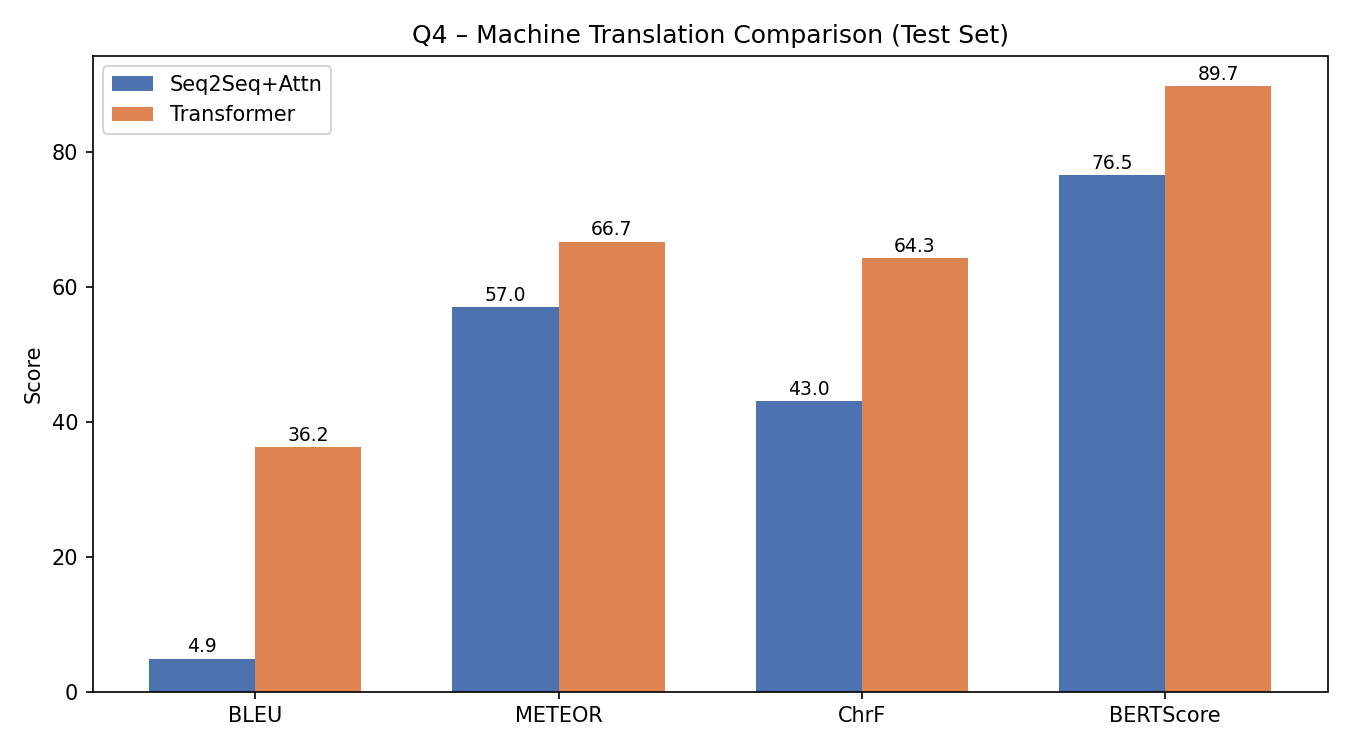
\includegraphics[width=0.85\linewidth]{figures/q4_comparison.png}
    \caption{Metric comparison between Seq2Seq+Attention and Helsinki
             Transformer on the Multi30k test set.}
    \label{fig:q4_comparison}
\end{figure}

\begin{figure}[H]
    \centering
    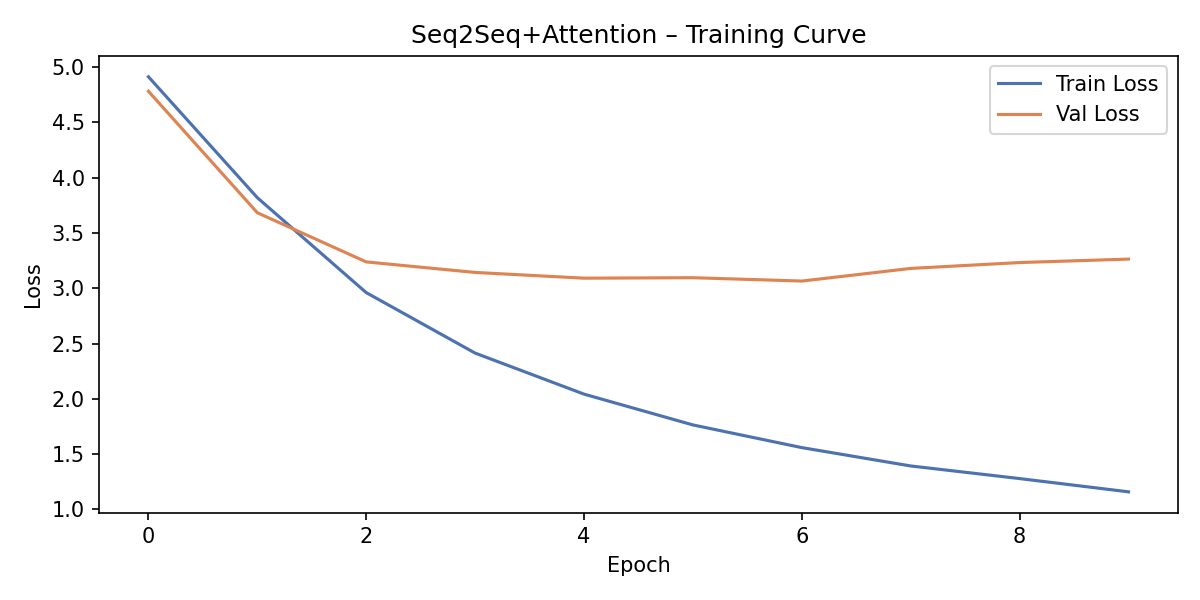
\includegraphics[width=0.75\linewidth]{figures/q4_s2s_training.png}
    \caption{Seq2Seq+Attention training and validation loss over 10 epochs.
             Overfitting begins from epoch 4 onward.}
    \label{fig:q4_s2s_train}
\end{figure}

\subsection{Qualitative Example}

\begin{table}[H]
    \centering
    \caption{Translation Examples from the Multi30k Test Set}
    \begin{tabular}{lp{9.5cm}}
        \toprule
        & \textbf{Example 1} \\
        \midrule
        Source (EN)    & A man in an orange hat starring at something. \\
        Reference (DE) & Ein Mann mit einem orangefarbenen Hut, der etwas anstarrt. \\
        Seq2Seq        & ein mann mit einem orangefarbenen hut starrt etwas etwas an . \\
        Transformer    & Ein Mann in einem orangenen Hut, der mit etwas zu tun hat. \\
        \midrule
        & \textbf{Example 2} \\
        \midrule
        Source (EN)    & A Boston Terrier is running on lush green grass in front of a white fence. \\
        Reference (DE) & Ein Boston Terrier l\"{a}uft \"{u}ber saftig-gr\"{u}nes Gras vor einem wei{\ss}en Zaun. \\
        Seq2Seq        & ein \texttt{<unk>} hirtenhund rennt auf gr\"{u}nes gr\"{u}nes gras vor einem wei{\ss}en zaun . \\
        Transformer    & Ein Boston Terrier l\"{a}uft auf \"{u}ppig gr\"{u}nem Gras vor einem wei{\ss}en Zaun. \\
        \midrule
        & \textbf{Example 3} \\
        \midrule
        Source (EN)    & A girl in karate uniform breaking a stick with a front kick. \\
        Reference (DE) & Ein M\"{a}dchen in einem Karateanzug bricht ein Brett mit einem Tritt. \\
        Seq2Seq        & ein m\"{a}dchen in \texttt{<unk>} wird einen einem mit einem stock . \\
        Transformer    & Ein M\"{a}dchen in Karate-Uniform bricht einen Stock mit einem Front-Kick. \\
        \bottomrule
    \end{tabular}
    \label{tab:q4_example}
\end{table}

In Example 2, Seq2Seq could not translate ``Boston Terrier'' because it was
outside its small vocabulary, so it produced \texttt{<unk>} and then guessed
``Hirtenhund'' (shepherd dog), which is completely wrong. In Example 3, the
output ``wird einen einem'' is grammatically incoherent, showing that the model
could not handle the morphological agreement rules of German. The Transformer
handled both cases correctly.

\subsection{Discussion}

The Transformer outperformed Seq2Seq on all metrics by a large margin.

\textbf{BLEU} (4.94 vs.\ 36.24) is the harshest metric here because it requires
exact word matches. Seq2Seq's many \texttt{<unk>} tokens and word repetitions
(e.g., ``grünes grünes'') severely hurt its BLEU score.

\textbf{METEOR} (56.97 vs.\ 66.68) is more forgiving thanks to stemming and
synonym matching. Seq2Seq still gets partial credit when it produces the right
root word even if the inflection is wrong.

\textbf{ChrF} (43.04 vs.\ 64.25) works at the character level, which is useful
for German because of its many inflected word forms. The Transformer scored much
higher here as well.

\textbf{BERTScore} (76.45 vs.\ 89.66) shows that even the weak Seq2Seq model
produces semantically relevant output most of the time. This suggests that the
model learned some meaningful word associations, even if the word forms and
order are often wrong.

The training curve (Figure~\ref{fig:q4_s2s_train}) shows clear overfitting
from epoch 4 onward. Training on only 29{,}000 sentence pairs is simply not
enough to learn the complexity of German. The Transformer, pre-trained on
millions of sentence pairs, had a huge head start.

% ════════════════════════════════════════════════════════════════════════════
\section{Language Modeling}
% ════════════════════════════════════════════════════════════════════════════

\subsection{Dataset Description}

The WikiText-2 dataset \cite{merity2016wikitext} was used. It consists of
Wikipedia articles and is a standard benchmark for language modeling. Compared
to Penn Treebank, it has a larger vocabulary and longer documents.

\begin{table}[H]
    \centering
    \caption{WikiText-2 Dataset Statistics}
    \begin{tabular}{lcc}
        \toprule
        \textbf{Split} & \textbf{Sentences} & \textbf{Tokens} \\
        \midrule
        Train      & 17{,}556 & 2{,}007{,}146 \\
        Validation &  1{,}841 &   209{,}338   \\
        Test       &  2{,}183 &   235{,}845   \\
        \bottomrule
    \end{tabular}
    \label{tab:q5_dataset}
\end{table}

A vocabulary of 10{,}000 tokens was built from the training set. Section
headings were excluded. Words outside the vocabulary were mapped to
\texttt{<unk>}.

\subsection{Model Implementations}

\subsubsection{Bigram Language Model}

A bigram model predicts each word given only the previous word:
$P(w_i \mid w_{i-1})$. Laplace (add-one) smoothing ($\alpha = 1.0$) was
applied to handle unseen word pairs. This model is count-based and requires
no training.

\subsubsection{Trigram Language Model}

A trigram model conditions on the two previous words:
$P(w_i \mid w_{i-2}, w_{i-1})$. The same Laplace smoothing was applied. While
theoretically capturing more context, it is much more affected by data sparsity,
as explained in the Discussion.

\subsubsection{LSTM Language Model}

A two-layer LSTM \cite{hochreiter1997lstm} was implemented. Token embeddings of
dimension 512 were fed into two LSTM layers with hidden size 512. Weight tying
was applied between the embedding matrix and the output projection layer.
Dropout of 0.5 was used throughout. Training ran for 15 epochs using SGD
(initial lr = 20.0), with learning rate halving from epoch 10 onward and
gradient clipping at 0.25. BPTT window size was 35, batch size 64. The model
has approximately 9.3M parameters.

\subsection{Results}

\begin{table}[H]
    \centering
    \caption{Language Model Perplexity (lower is better)}
    \begin{tabular}{lcc}
        \toprule
        \textbf{Model} & \textbf{Val.\ Perplexity} & \textbf{Test Perplexity} \\
        \midrule
        Bigram             & 1{,}473.88 & 1{,}504.73 \\
        Trigram            & 5{,}287.55 & 5{,}341.04 \\
        \textbf{LSTM}      & \textbf{70.52}  & \textbf{66.77}  \\
        \bottomrule
    \end{tabular}
    \label{tab:q5_results}
\end{table}

\begin{figure}[H]
    \centering
    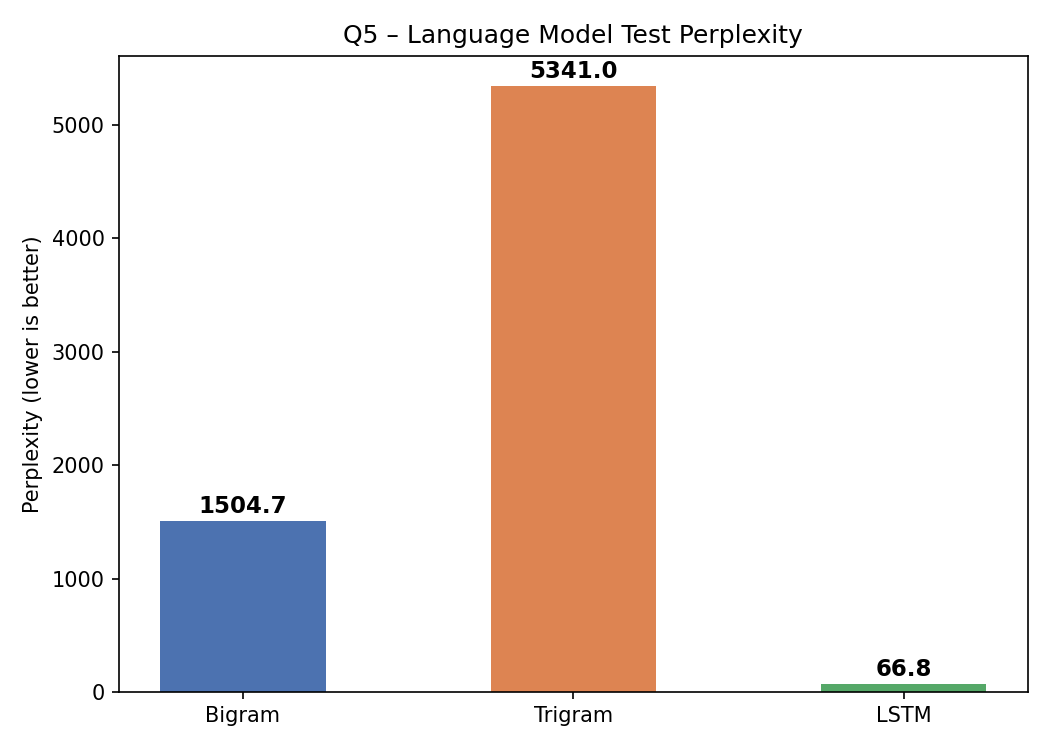
\includegraphics[width=0.70\linewidth]{figures/q5_comparison.png}
    \caption{Test perplexity comparison across the three language models.}
    \label{fig:q5_comparison}
\end{figure}

\begin{figure}[H]
    \centering
    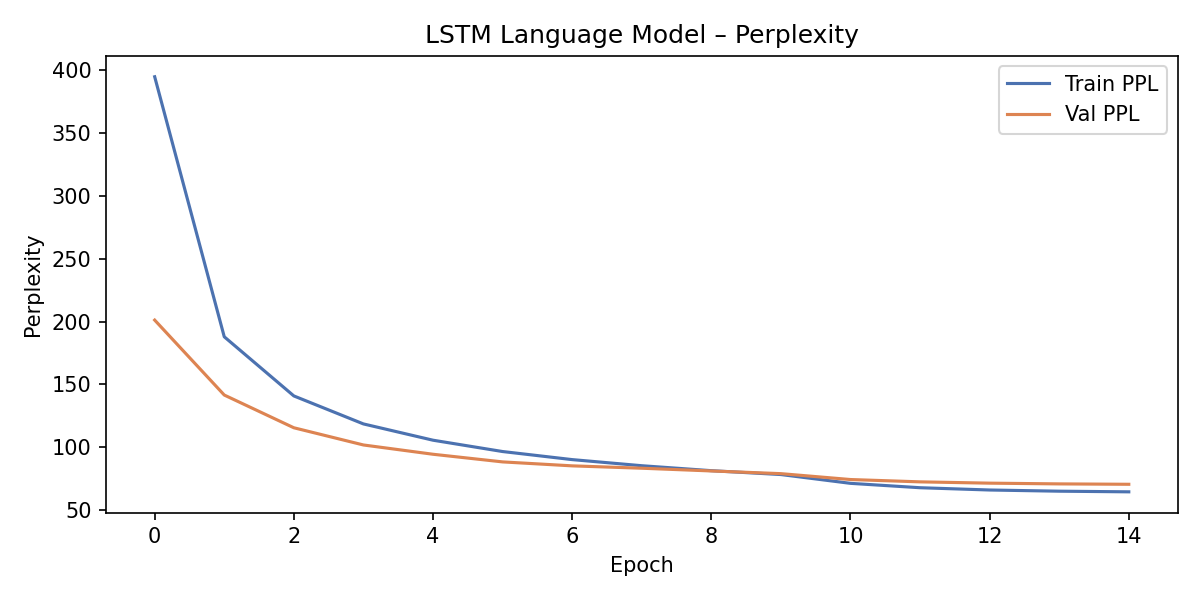
\includegraphics[width=0.75\linewidth]{figures/q5_lstm_training.png}
    \caption{LSTM training and validation perplexity over 15 epochs.
             Learning rate decay from epoch 10 accelerates convergence.}
    \label{fig:q5_lstm_train}
\end{figure}

\subsection{Generated Text Samples}

\begin{table}[H]
    \centering
    \caption{Generated Text Samples (seed words in bold)}
    \begin{tabular}{lp{10cm}}
        \toprule
        \textbf{Model} & \textbf{Generated Text} \\
        \midrule
        Bigram  &
        \textbf{the} canadian / soul of the local tradition by dave thomas 's
        misdirected martyrdom of the 1st , that " a \\[4pt]
        Bigram  &
        \textbf{he} was able to mogadishu . \\[4pt]
        \midrule
        Trigram &
        \textbf{the} junta to become the show received a message back for more
        than one cult center , which travels to sarasaland \\[4pt]
        Trigram &
        \textbf{he} nails it " her two elder pitman children received their
        offerings in bodies of the 2004 mtv video music awards \\[4pt]
        \midrule
        LSTM    &
        \textbf{the} \texttt{<unk>} \texttt{<unk>} and the \texttt{<unk>}
        of the \texttt{<unk>} . \\[4pt]
        LSTM    &
        \textbf{he was} the only choice of the history of the city . \\
        \bottomrule
    \end{tabular}
    \label{tab:q5_samples}
\end{table}

\subsection{Discussion}

\textbf{Perplexity results.}
The LSTM dramatically outperformed both n-gram models, reaching a test
perplexity of 66.77 compared to 1{,}504.73 for Bigram and 5{,}341.04 for Trigram.

The most surprising finding was that the Trigram performed \textit{worse} than
the Bigram, even though it uses more context. The reason is data sparsity
combined with Laplace smoothing. With a 10{,}000-word vocabulary, there are
$10{,}000^2 = 10^8$ possible trigram contexts — far more than actually appear in
the training data. Laplace smoothing adds $\alpha \cdot V$ counts to the
denominator of every context, which effectively pushes all probabilities toward
uniform. Kneser-Ney smoothing would handle this much better.

\textbf{Training dynamics.}
The LSTM's perplexity curve (Figure~\ref{fig:q5_lstm_train}) drops quickly in
the first five epochs and then continues to improve steadily after learning rate
decay kicks in at epoch 10. Importantly, training and validation curves stay
close to each other throughout — there is no sign of overfitting. This is thanks
to the high dropout (0.5) and weight tying.

\textbf{Generation quality.}
Bigram outputs are locally plausible (e.g., ``he was able to...'') but jump
between unrelated topics from word to word. Trigram outputs are slightly more
coherent in short spans but are still semantically disconnected overall. LSTM
outputs suffer from many \texttt{<unk>} tokens because the 10{,}000-token
vocabulary is much smaller than WikiText-2's full 33{,}000-token vocabulary.
However, the ``he was'' sample produced a grammatically correct and meaningful
sentence, showing the LSTM has learned real language structure.

\textbf{Summary.}
N-gram models are fast and need no GPU, but they are severely limited by data
sparsity and the Markov assumption. The LSTM overcomes both problems by learning
dense representations and capturing long-range dependencies, though it requires
more resources and training time.



% ════════════════════════════════════════════════════════════════════════════
\newpage
\bibliographystyle{plain}
\bibliography{references}
\end{document}